\documentclass{article}
\usepackage{graphicx} % Required for inserting images
\usepackage{float}
\usepackage[T1]{fontenc}
\usepackage{amsmath}
\usepackage[margin=1in]{geometry}
\usepackage{booktabs}
\usepackage{tabularx}
\usepackage[hidelinks]{hyperref}

\title{Selling a 20-delta put instead of a 25-delta put, on the stress-sized put book}
\author{Experiment report \textperiodcentered{} L/S Gamma Desk, QUANTT}
\date{2026-11-02}

\begin{document}

\maketitle

\textbf{Question:} On the 35\% stress-sized \texttt{hedged} book, does selling the 20-delta put instead of the 25-delta put earn more net P\&L, at 1x and 2x spreads, without a worse tail or a drawdown beyond the stress budget?

\textbf{Method:}

\begin{itemize}

\item \textbf{Pre-registered backtest:} the hypothesis card was committed before any run (commit bc7506b). The batch's research switches were committed before it (a2d5334); this card needs none of them.

\item \textbf{Data:} the live paper rules (\texttt{configs/\allowbreak{}paper.\allowbreak{}toml}) are replayed on R2 replay snapshots v1 (config\_hash b040760187f0) over the development window 2014-06-02 to 2024-12-31. The hold-out (2025-01-01 to 2026-07-10) was not used.

\item \textbf{Book (every variant and the reference):} the \texttt{hedged} book of \texttt{2026-\allowbreak{}10-\allowbreak{}22-\allowbreak{}stress-\allowbreak{}sized-\allowbreak{}puts}.

\begin{itemize}

\item An always-on short put, with the signal ignored and the flat exit off.

\item Sized at entry so that a one-day 20\% SPY drop, with IV at max(60\%, the put's IV), costs at most 35\% of \$250k (\$87,500).

\item A 10-share daily hedge.

\item The 1x-credit stop, the 50\% profit-take, the 7-DTE time exit and the 1-day cool-off.

\end{itemize}

\item \textbf{Variants:} the strike is the listed put with delta closest to the target, on the expiry closest to 30 DTE within 21-45 DTE (existing switch \texttt{[backtest] put\_\allowbreak{}delta}).

\begin{itemize}

\item \texttt{put20} (primary): \texttt{put\_\allowbreak{}delta = 0.\allowbreak{}20};

\item \texttt{put15} (sensitivity): \texttt{put\_\allowbreak{}delta = 0.\allowbreak{}15}.

\end{itemize}

\item \textbf{Comparison:} the registered \texttt{2026-\allowbreak{}10-\allowbreak{}22-\allowbreak{}stress-\allowbreak{}sized-\allowbreak{}puts/\allowbreak{}hedged} runs (25-delta) at the same spread multiple, reused and not rerun.

\item \textbf{Runs and costs:}

\begin{itemize}

\item Every variant was run at 1x and 2x spreads.

\item Costs are \$0.65 per contract and \$0.005 per share, with a \$1 minimum per order.

\end{itemize}

\item \textbf{Timing:}

\begin{itemize}

\item Decisions, exits and hedges run at 10:15 ET.

\item Decisions read a 15-minute-old chain, and fills price on trades in the 15 minutes after.

\item Spot comes from put-call parity on the 30-minute snapshot grid (10:15-15:45).

\end{itemize}

\end{itemize}

This report was written by Claude at the PM's request.

\section{Result vs the pass bar}

Every check had to hold at 1x and 2x. P\&L is net of costs in USD for the whole sized book. ES is the mean of the worst 5\% of daily P\&L.

\begin{center}\small
\begin{tabularx}{\linewidth}{>{\raggedright\arraybackslash}X l l l l l}
\toprule
\textbf{Check (\texttt{put20} vs \texttt{hedged})} & \textbf{1x value} & \textbf{1x bar} & \textbf{2x value} & \textbf{2x bar} & \textbf{Result} \\
\midrule
Net P\&L, full window & \$149,893 & > \$121,482 & \$133,123 & > \$101,172 & pass \\
Net P\&L, 2014-06 to 2019-12 & \$59,301 & > \$49,132 & \$50,199 & > \$42,687 & pass \\
Net P\&L, 2020-01 to 2024-12 & \$90,592 & > \$72,350 & \$82,924 & > \$58,485 & pass \\
ES 5\% within 1.10x & \ensuremath{-}\$2,457 & \ensuremath{\geq} \ensuremath{-}\$3,317 & \ensuremath{-}\$2,489 & \ensuremath{\geq} \ensuremath{-}\$3,404 & pass \\
Max drawdown \ensuremath{\leq} \$87,500 & \$48,435 & \ensuremath{\leq} \$87,500 & \$51,352 & \ensuremath{\leq} \$87,500 & pass \\
Event floor: round trips \ensuremath{\geq} 30 & 192 & \ensuremath{\geq} 30 &  &  & met \\
\bottomrule
\end{tabularx}
\end{center}

\textbf{Verdict: passed (in-sample).}

\begin{itemize}

\item \texttt{put20} made \$28k more than the 25-delta book at 1x and \$32k more at 2x, with a higher Sharpe (0.78 against 0.52 at 1x), a smaller drawdown and a milder tail.

\item But the lead is concentrated. One month, August 2015, gives \$26.5k of the \$28.4k lead at 1x. On the 92 entry days the two books share, the 20-delta put earned no more per contract.

\item The analysis below explains why the result is mostly a change in the book's roll calendar, not a better strike.

\end{itemize}

\subsection{Full-window numbers (not part of the bar)}

\begin{center}\small
\begin{tabularx}{\linewidth}{>{\raggedright\arraybackslash}X >{\raggedright\arraybackslash}X >{\raggedright\arraybackslash}X >{\raggedright\arraybackslash}X >{\raggedright\arraybackslash}X >{\raggedright\arraybackslash}X >{\raggedright\arraybackslash}X}
\toprule
\textbf{} & \textbf{hedged 1x} & \textbf{put20 1x} & \textbf{put15 1x} & \textbf{hedged 2x} & \textbf{put20 2x} & \textbf{put15 2x} \\
\midrule
Net P\&L & \$121,482 & \$149,893 & \$113,809 & \$101,172 & \$133,123 & \$110,501 \\
Sharpe & 0.52 & 0.78 & 0.47 & 0.43 & 0.69 & 0.45 \\
Max drawdown & \$70,362 & \$48,435 & \$77,832 & \$75,488 & \$51,352 & \$83,114 \\
ES 5\% (daily) & \ensuremath{-}\$3,016 & \ensuremath{-}\$2,457 & \ensuremath{-}\$2,575 & \ensuremath{-}\$3,094 & \ensuremath{-}\$2,489 & \ensuremath{-}\$2,584 \\
Round trips & 182 & 192 & 194 & 181 & 190 & 196 \\
Commissions (options /\allowbreak{} hedges) & \$5,955 /\allowbreak{} \$2,868 & \$6,248 /\allowbreak{} \$2,659 & \$6,403 /\allowbreak{} \$2,458 & \$5,918 /\allowbreak{} \$2,863 & \$6,156 /\allowbreak{} \$2,646 & \$6,527 /\allowbreak{} \$2,455 \\
\bottomrule
\end{tabularx}
\end{center}

\texttt{put15} failed the same bar (it trails over the full window at 1x and in 2014-2019 at both spreads), so the effect does not grow as the delta falls.

\section{Charts}

\begin{figure}[H]\centering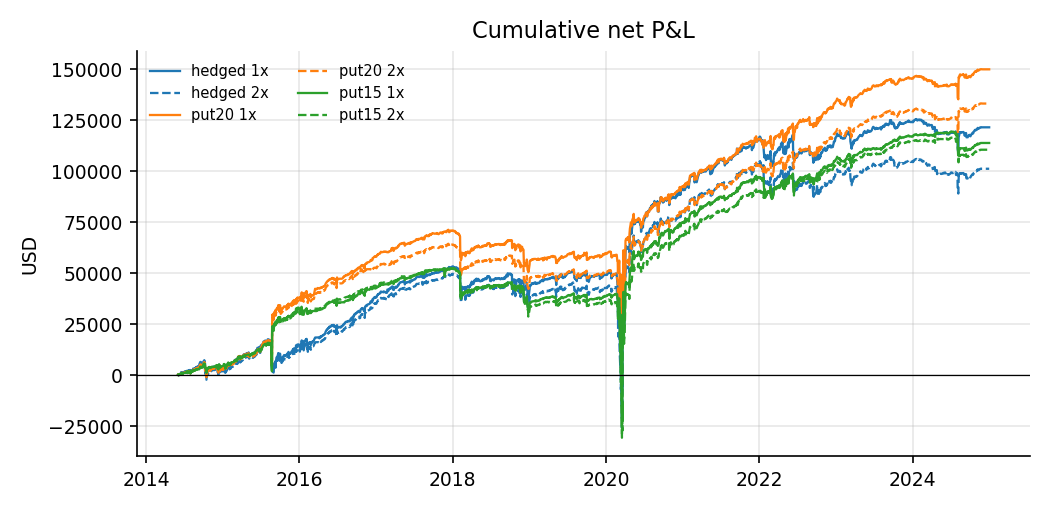
\includegraphics[width=0.92\linewidth]{figures/cum_pnl.png}\caption{Cumulative net P\&L, 1x solid and 2x dashed}\end{figure}

\texttt{put20} jumps ahead in August 2015 (\$26.5k at 1x by end-August), gives that lead back by 2021 (\$10.2k at end-2019, \$1.4k at end-2020, \ensuremath{-}\$0.3k at end-2021), and regains it in 2022-2024 (+\$28.7k).

\begin{figure}[H]\centering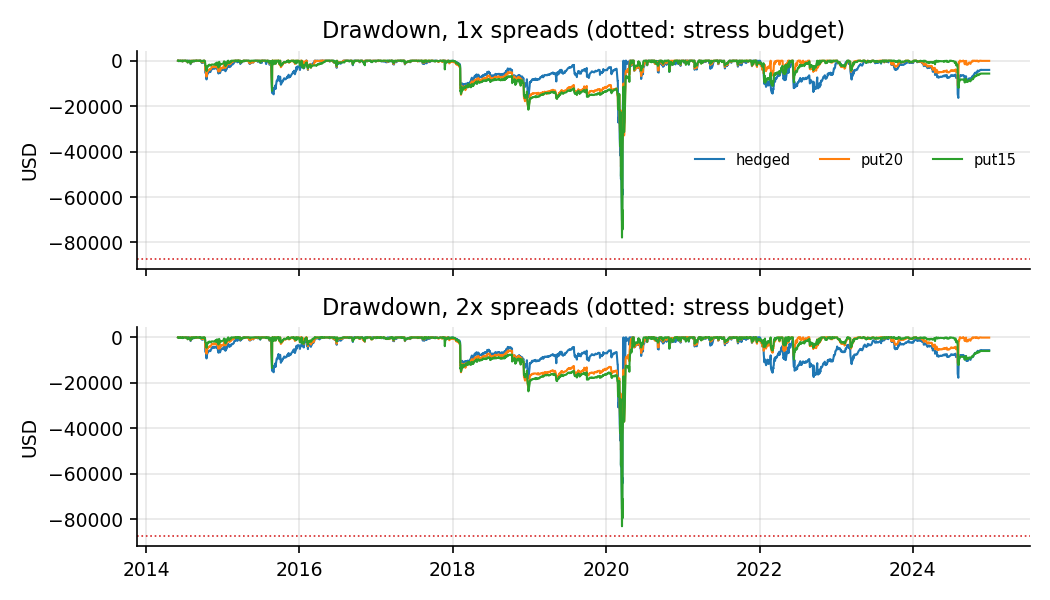
\includegraphics[width=0.92\linewidth]{figures/drawdown.png}\caption{Drawdown at 1x and 2x spreads}\end{figure}

Every book's deepest drawdown is March 2020, and every book stays inside the \$87,500 budget (dotted):

\begin{itemize}

\item \texttt{hedged}: \$70k;

\item \texttt{put20}: \$48k;

\item \texttt{put15}: \$78k.

\end{itemize}

The difference between \texttt{hedged} and \texttt{put20} comes from different paths through that month, analysed below.

\begin{figure}[H]\centering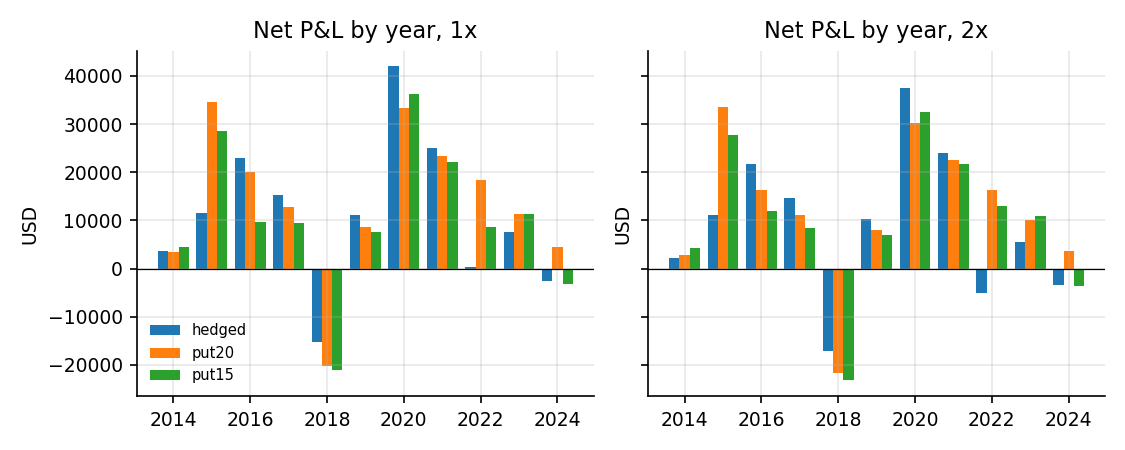
\includegraphics[width=0.92\linewidth]{figures/yearly.png}\caption{Net P\&L by year}\end{figure}

\texttt{put20} is ahead in 2015, 2022, 2023 and 2024 at 1x, and behind in the other seven years, by \$0.2k-8.7k each. The two large gains (2015 +\$23.1k, 2022 +\$17.9k at 1x) are each one or two episodes.

\begin{figure}[H]\centering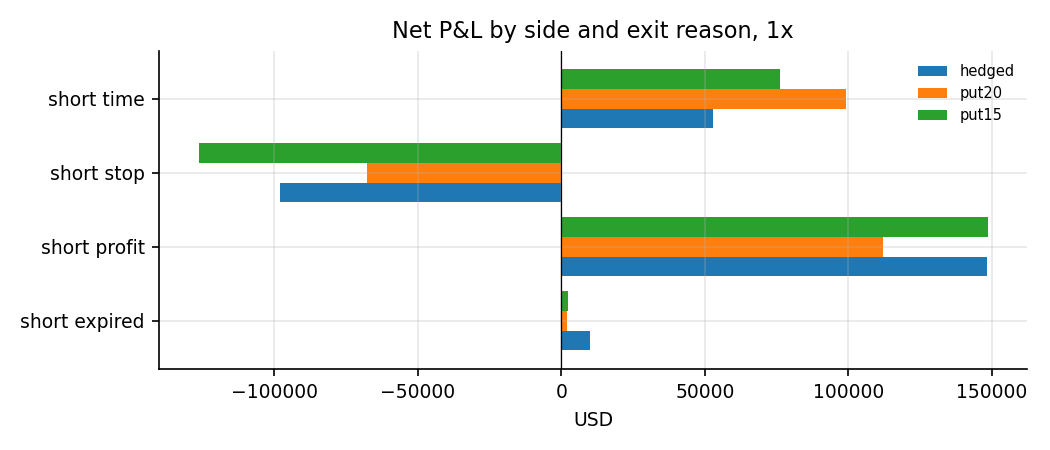
\includegraphics[width=0.92\linewidth]{figures/by_reason.png}\caption{Net P\&L by side and exit reason, 1x}\end{figure}

The lower-delta books take profit and stop out more often. Out of round trips (expiries not shown: 2, 2 and 6):

\begin{center}\small
\begin{tabularx}{\linewidth}{l l l >{\raggedright\arraybackslash}X}
\toprule
\textbf{} & \textbf{profit-takes} & \textbf{stops} & \textbf{time exits} \\
\midrule
\texttt{hedged} & 25 & 8 & 147 \\
\texttt{put20} & 39 & 14 & 137 \\
\texttt{put15} & 51 & 19 & 118 \\
\bottomrule
\end{tabularx}
\end{center}

\texttt{put20}'s stops lost less in total than the reference's.

\begin{figure}[H]\centering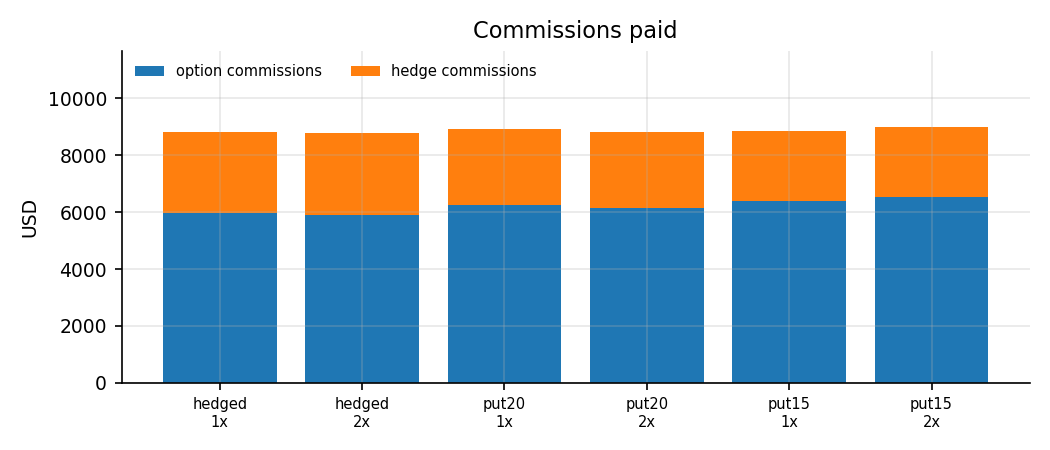
\includegraphics[width=0.92\linewidth]{figures/fees.png}\caption{Commissions paid}\end{figure}

Commissions are about \$8.8-8.9k in every book: lower-delta books pay slightly more on options and slightly less on hedges.

\begin{figure}[H]\centering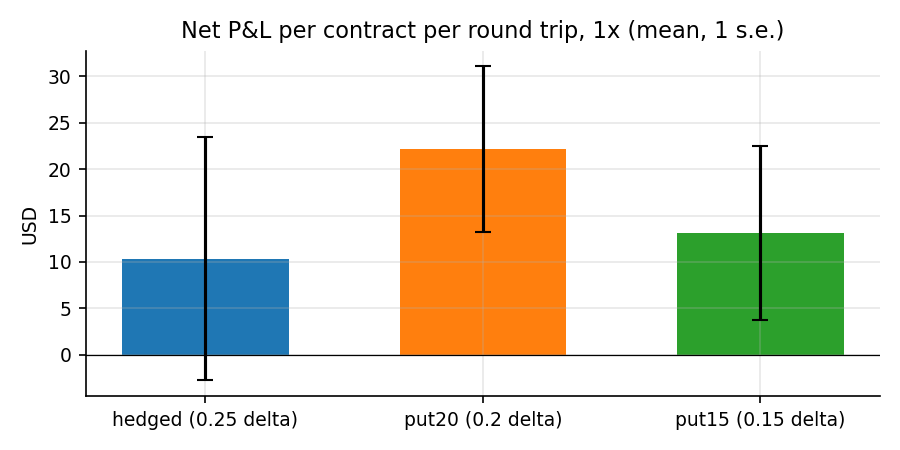
\includegraphics[width=0.92\linewidth]{figures/per_contract.png}\caption{Net P\&L per contract per round trip, 1x (mean, 1 s.e.)}\end{figure}

The mean per-contract net is \$10.3 for the reference, \$22.1 for \texttt{put20} and \$13.1 for \texttt{put15}. The standard errors are \$9-13, so the differences are within noise. Pooled over contracts the figures are \$24.5, \$30.0 and \$20.1.

\begin{figure}[H]\centering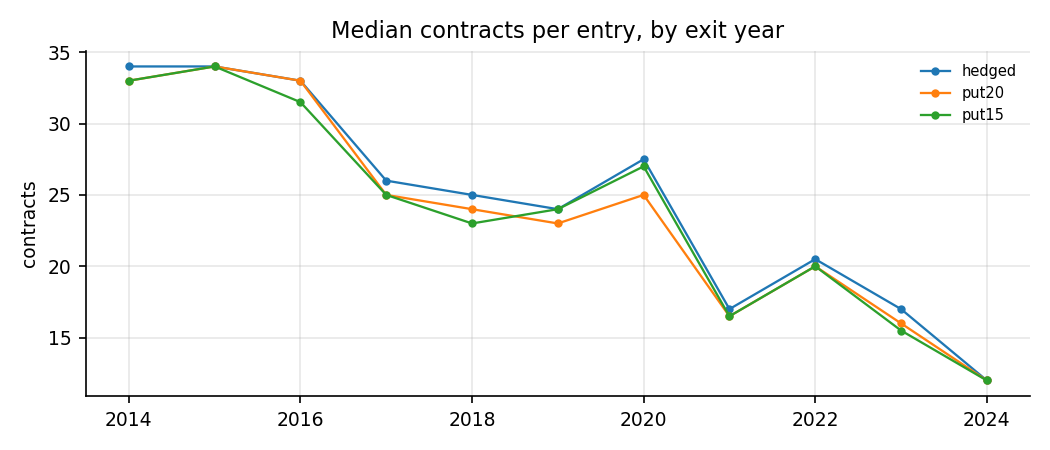
\includegraphics[width=0.92\linewidth]{figures/contracts.png}\caption{Median contracts per entry, by exit year}\end{figure}

The stress budget sizes all three books almost the same: means of 25.4, 25.2 and 25.9 contracts. The reason is that in a 20\% drop with IV at 60\% or more, all three puts are deep in the money, so their stress losses are close. A lower-delta put therefore does not buy more contracts. It just collects less premium per contract: about \$265, \$210 and \$153 on average.

\begin{figure}[H]\centering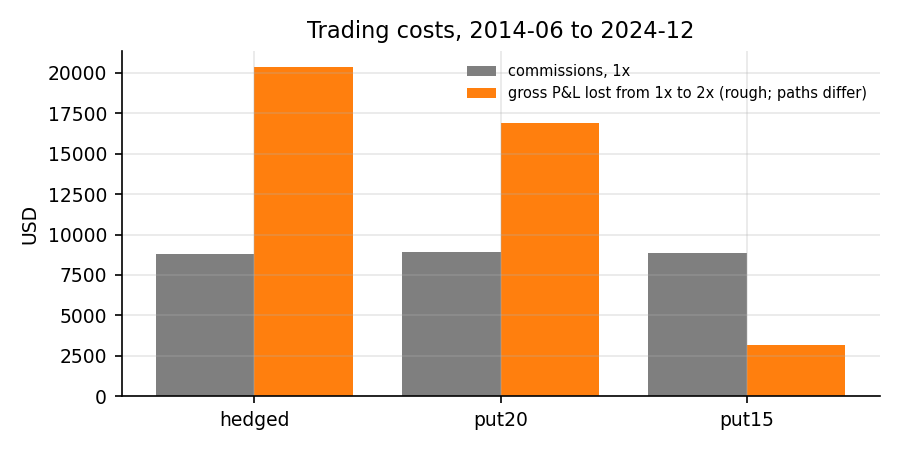
\includegraphics[width=0.92\linewidth]{figures/costs.png}\caption{Trading costs}\end{figure}

The orange bar is the gross P\&L lost going from 1x to 2x spreads, a rough stand-in for the spread paid at 1x. It is not reliable here: the 1x and 2x runs take slightly different paths. \texttt{put15}'s \$3.2k is mostly that path effect, not a cheaper option.

\section{Analysis}

\textbf{The lead comes from the path, not the strike.}

\begin{itemize}

\item Only 92 of the reference's 182 entries fall on the same day as one of \texttt{put20}'s.

\item On those 92 shared entry days, the books earned almost the same: \texttt{put20} \$70.0k against \$71.7k for the reference at 1x, \$31.0 against \$31.2 per contract.

\item The whole lead comes from trades entered on different days.

\end{itemize}

The mechanism is mechanical. A lower-delta put reaches its 50\% profit-take and its 1x-credit stop at different times from a 25-delta put, so the book closes and re-enters on a different calendar. After a few months the two books roll on different days. Which calendar happens to sit through a selloff then decides the result.

\textbf{August 2015 decides most of it.}

\begin{center}\small
\begin{tabularx}{\linewidth}{>{\raggedright\arraybackslash}X >{\raggedright\arraybackslash}X >{\raggedright\arraybackslash}X}
\toprule
\textbf{} & \textbf{\texttt{hedged}} & \textbf{\texttt{put20}} \\
\midrule
Stopped out & Monday 24 August (the flash-crash open) & Friday 21 August \\
Re-entry & 25 August, 51 contracts & 24 August at 10:15, at very high IV: 104 contracts, the stress rule sizing up \\
That re-entry &  & took its profit two days later, +\$14.9k \\
August 2015 net P\&L, 1x & \ensuremath{-}\$13.5k & +\$12.9k \\
\bottomrule
\end{tabularx}
\end{center}

Excluding August 2015, the two books are close:

\begin{itemize}

\item 1x: \$136.9k against \$135.0k;

\item 2x: \$120.5k against \$115.4k.

\end{itemize}

\textbf{Other episodes:}

\begin{itemize}

\item \textbf{March 2020.} \texttt{put20} was stopped on 27 February and re-entered on 28 February with 54 contracts. That put was never stopped: it closed at its time exit on 20 March, +\$12.9k. So the book avoided the reference's stops on 28 February and 12 March, which is why its drawdown is \$48k rather than \$70k. It also missed the reference's 100-contract sale on 13 March: from 19 February to 30 April 2020, \texttt{put20} made \$15.9k against \$21.7k.

\item \textbf{June 2022.} The reference's put opened on 27 May lost \$15.9k in the mid-June selloff. \texttt{put20}'s calendar had it in a fresh put from 10 June, which made money. That gap is \$7.8k of the 2022 difference.

\end{itemize}

\textbf{Outside these episodes, the 20-delta book trails slightly.}

\begin{itemize}

\item \texttt{put20} is ahead in 59 of 127 months.

\item Excluding 2015 and 2022, it made \$97.0k against \$109.6k at 1x.

\item That is consistent with lower premium per contract at the same size, offset by fewer costly stops in large selloffs.

\end{itemize}

\textbf{\texttt{put15} does not confirm it.} It also gains in August 2015 (+\$8.8k against \ensuremath{-}\$13.5k), but less, and it fails the bar. That makes it hard to read the result as ``lower delta is better''.

\textbf{What is mechanical, and what may be noise:}

\begin{itemize}

\item Mechanical:

\begin{itemize}

\item equal sizing across deltas, since the stress test is dominated by intrinsic value;

\item lower premium per contract;

\item more profit-takes and stops.

\end{itemize}

\item Path-dependent, and so possibly noise: the P\&L lead. It rests on the timing of one re-entry in August 2015 and on two other roll-calendar accidents.

\end{itemize}

\section{Verdict}

\textbf{Passed} on the pre-registered bar at 1x and 2x, in-sample. The bar was met by a margin, but most of the margin is August 2015 (one stale-view crash-day re-entry and a well-timed stop). That lead was fully given back by 2021 and rebuilt in 2022-2024, and on shared entry days the strike made no difference. The next step is the PM's: a hold-out run of \texttt{put20} (\texttt{/\allowbreak{}run-\allowbreak{}experiment-\allowbreak{}with-\allowbreak{}report holdout 2026-\allowbreak{}11-\allowbreak{}02-\allowbreak{}lower-\allowbreak{}delta}). It needs the 2026-10-22 \texttt{hedged} hold-out run as its reference, which is that card's single hold-out look, so the PM would decide both together. Don't expect the in-sample margin to repeat.

\section{Caveats}

\begin{itemize}

\item \textbf{In-sample.} The idea comes from the 2026-10-22 deep research, written after the desk's 25-delta, 35-delta and ATM results on 2014-2024. Before pre-registration, Claude saw the reference book's aggregate trip and cost figures while testing the reporting code (stated in the card).

\item \textbf{Concentration.} One month gives 93\% of the 1x lead. The roll calendars of the two books overlap on only half the entries.

\item \textbf{Spread model.} It was fitted on about two weeks of calm 2026 live quotes; the 2x run is the stress test. Fills of 50-100 contracts on crash days use the same one-contract model, and the 104-contract entry on 24 August 2015 is the kind of fill it may flatter. The engine sized that entry on the 15-minute-stale decision view taken near the crash low; SPY had rallied by the fill view, where the same rule would have sized 87 contracts. Because the position is marked at the decision view on entry day, \texttt{put20} shows an \$8.1k loss on 24 August that reverses the next day. This is the engine working as designed (a live run faces the same lag), but it is part of why the trade was so large.

\item \textbf{Stress model.} Black-Scholes, with no IV shock above max(60\%, IV). That is why the deltas size alike.

\item \textbf{Margin.} Not modelled.

\item \textbf{Data gaps.} About 3.3\% of scheduled times are skipped (no R2 data), and 0.4-1.4\% of hedge times have no delta for the held put (0.4\% for \texttt{put20} at 1x).

\end{itemize}

\section{Trials}

\begin{itemize}

\item 4 trials for this experiment: 2 variants \ensuremath{\times} 1x and 2x, one run of \texttt{experiment.\allowbreak{}py}.

\item The reference \texttt{2026-\allowbreak{}10-\allowbreak{}22-\allowbreak{}stress-\allowbreak{}sized-\allowbreak{}puts/\allowbreak{}hedged} and the baseline's 2 trials were reused, not rerun.

\item \textbf{\texttt{-\allowbreak{}dirty} tags.} The registry tags the runs \texttt{af47198-\allowbreak{}dirty} (\texttt{put20} 1x) and \texttt{3568520-\allowbreak{}dirty} (the other three).

\begin{itemize}

\item Those are later pre-registration commits of other cards in the same batch, which contain this card's pre-registration bc7506b. Between bc7506b and those commits, the engine, the configs and this card's files did not change.

\item The dirty flag comes from other cards' uncommitted files in the shared working tree.

\end{itemize}

\item The cost chart's label was corrected and the figures rebuilt with \texttt{-\allowbreak{}-\allowbreak{}report-\allowbreak{}only}, which adds no trials.

\item The pass bar was not changed.

\end{itemize}

\end{document}
